\subsection{Background}
Image compression consists in encoding an image into a format that requires a lower storage space. If information stored in this format can then be used to obtain the original image, compression is denoted as lossless, otherwise it is called lossy. 

The need for image compression becomes self-evident when considering the following examples. Storing an image with 1080 by 1920 pixels, 3 color bands and 256 possible values for each color in an uncompressed format would require about 6. Even worse, storing a video with 30 frames per second and a duration of just 10 minutes would require 3.55 GB. 

For said reason, a large number of image compression techniques have been proposed\cite{compression_list_1}\cite{compression_list_2}\cite{compression_wavelet}, differing in compression rate, quality of the decoded image and execution time for compression and decompression. The interest for efficient image compression algorithms is high, and multiple works focus on improving the run time of existing algorithms or developing new ones\cite{compression_optimize_1}\cite{compression_optimize_2}.

Transform coding was introduced in the late 1960s, with the Discrete Cosine Transform (DCT) being introduced in 1972 by Nasir Ahmed\cite{dct}. JPEG\cite{jpeg}, the most widely used compression standard in the world\cite{jpeg_popular}, makes use of the DCT and techniques such as quantization and run-length encoding.

\subsection{Code structure and functionalities}
To test our understanding of the concepts behind image compression, we implemented a custom version of the JPEG standard, with the following differences:
\begin{itemize}
    \item JPEG uses the DCT, while we decided to use the DFT. While we established that the DCT is indeed more suitable for image compression, the fundamental idea of decomposing a signal into its constituent frequencies remains valid. Similary to the DCT, using the DFT to express the image as a sum of frequencies allowed us to discard the frequencies that the human eye is less sensitive to, and thus compress the image.
    \item JPEG uses the YCbCr color space, while we use the grayscale color space and only support grayscale images.
    \item We had to develop a custom quantization matrix due to the fact that a different transform is used.
    \item We use a simplified version of the run-length encoding scheme used in JPEG.
\end{itemize}

Most compression-related functionalities are declared in \texttt{Grayscale\-Image.hpp}, implemented in \texttt{Grayscale\-Image.cpp} and used in \texttt{compression\_\-main\-.cpp}. The \texttt{GrayscaleImage} class exposes functionalities for loading, storing and displaying an image using OpenCV, and to encode and decode images using our custom algorithm. Moverover, some wavelet-related functionalities are implemented, which will be described in Section \ref{sec:wavelet}.

The \texttt{encode} method of \texttt{Grayscale\-Image} consists in the following steps:
\begin{enumerate}
    \item Split the image into 8x8 blocks.
    \item Apply a 2D direct FFT to each block.
    \item Quantize the coefficients of each block, using a hand-made quantization matrix.
    \item Read the block in a zig-zag fashion and apply run-length encoding to the coefficients.
\end{enumerate}
Clearly, the \texttt{decode} method does the same steps backward, reconstructing the image up to the data that was lost due to the lossy compression.

\subsubsection{Applying the DFT}
Just like in JPEG, all pixel values are subtracted 128 to be mapped to the range [-128,127]. Then, a 2D direct FFT is applied to each block.

The implementation of the 2D FFT used in this method is the one provided in the class \texttt{Two\-Dimensional\-Direct\-FFT\-CPU}. The loop over the 8x8 blocks is parallelized using OpenMP, and each block is transformed using the algorithm provided in \texttt{Iterative\-Fourier\-Transform\-Algorithm} on each row and column. While the function could easily be changed to use the CUDA implementation, the reason for this choice is that most of the code for image compression had to be developed and tested on a machine without CUDA support. 

\subsubsection{Quantization}
JPEG uses a quantization table, which consists in a matrix of coefficients. Each pixel in a block is divided by the respective coefficient of the quantization table, resulting in a reduction in the range of the possible values of the coefficients. The values are then stored as an integer, causing values that are below 1 to be stored as 0. Clearly, this step is irreversible and is the main reason behind the lossy nature of the compression. Our implementation uses a custom version of the quantization table, as the original one was developed for the DCT and is inadequate for our algorithm. Moreover, since the result of the DCT is a sequence of real coefficients, while the result of the DFT is a sequence of complex coefficients, the quantization is performed for both the real and immaginary coefficients separately. Not knowing what the optimal values of the quantization table are for our algorithm, we set most values to 100, with the value in the top left set to 200, since it is the largest coefficient of the transformed sequence by far.

\subsubsection{Run-length encoding}
This step consists in storing the resulting values for the coefficients of each block using a zig-zag pattern and performing run-length encoding. This pattern is used because it has been shown that it increases the effectiveness of the encoding technique. To avoid recomputing the zig-zag pattern, it is stored as an array, as it always has exactly 64 elements. Our run-length encoding algorithm consists in storing each non-zero value explicitely, with non-zero values separated by the number of 0s between them. This algorithm is applied to both the real and the immaginary coefficients, which are then concatenated together.

\subsection{Results}
Figures \ref{fig:compression_road} and \ref{fig:compression_cat} show the results of compressing an image with our algorithm and then decompressing it. The first image is almost unchanged, while the second one shows some noise and artifacts. In particular, the fact that the image was split into 8x8 blocks can be clearly seen in Figure \ref{fig:compression_cat}, which is an issue that JPEG compression suffers from as well. 

\begin{figure}[ht]
    \centering
    \subfigure[Original image]{\label{fig:road_original}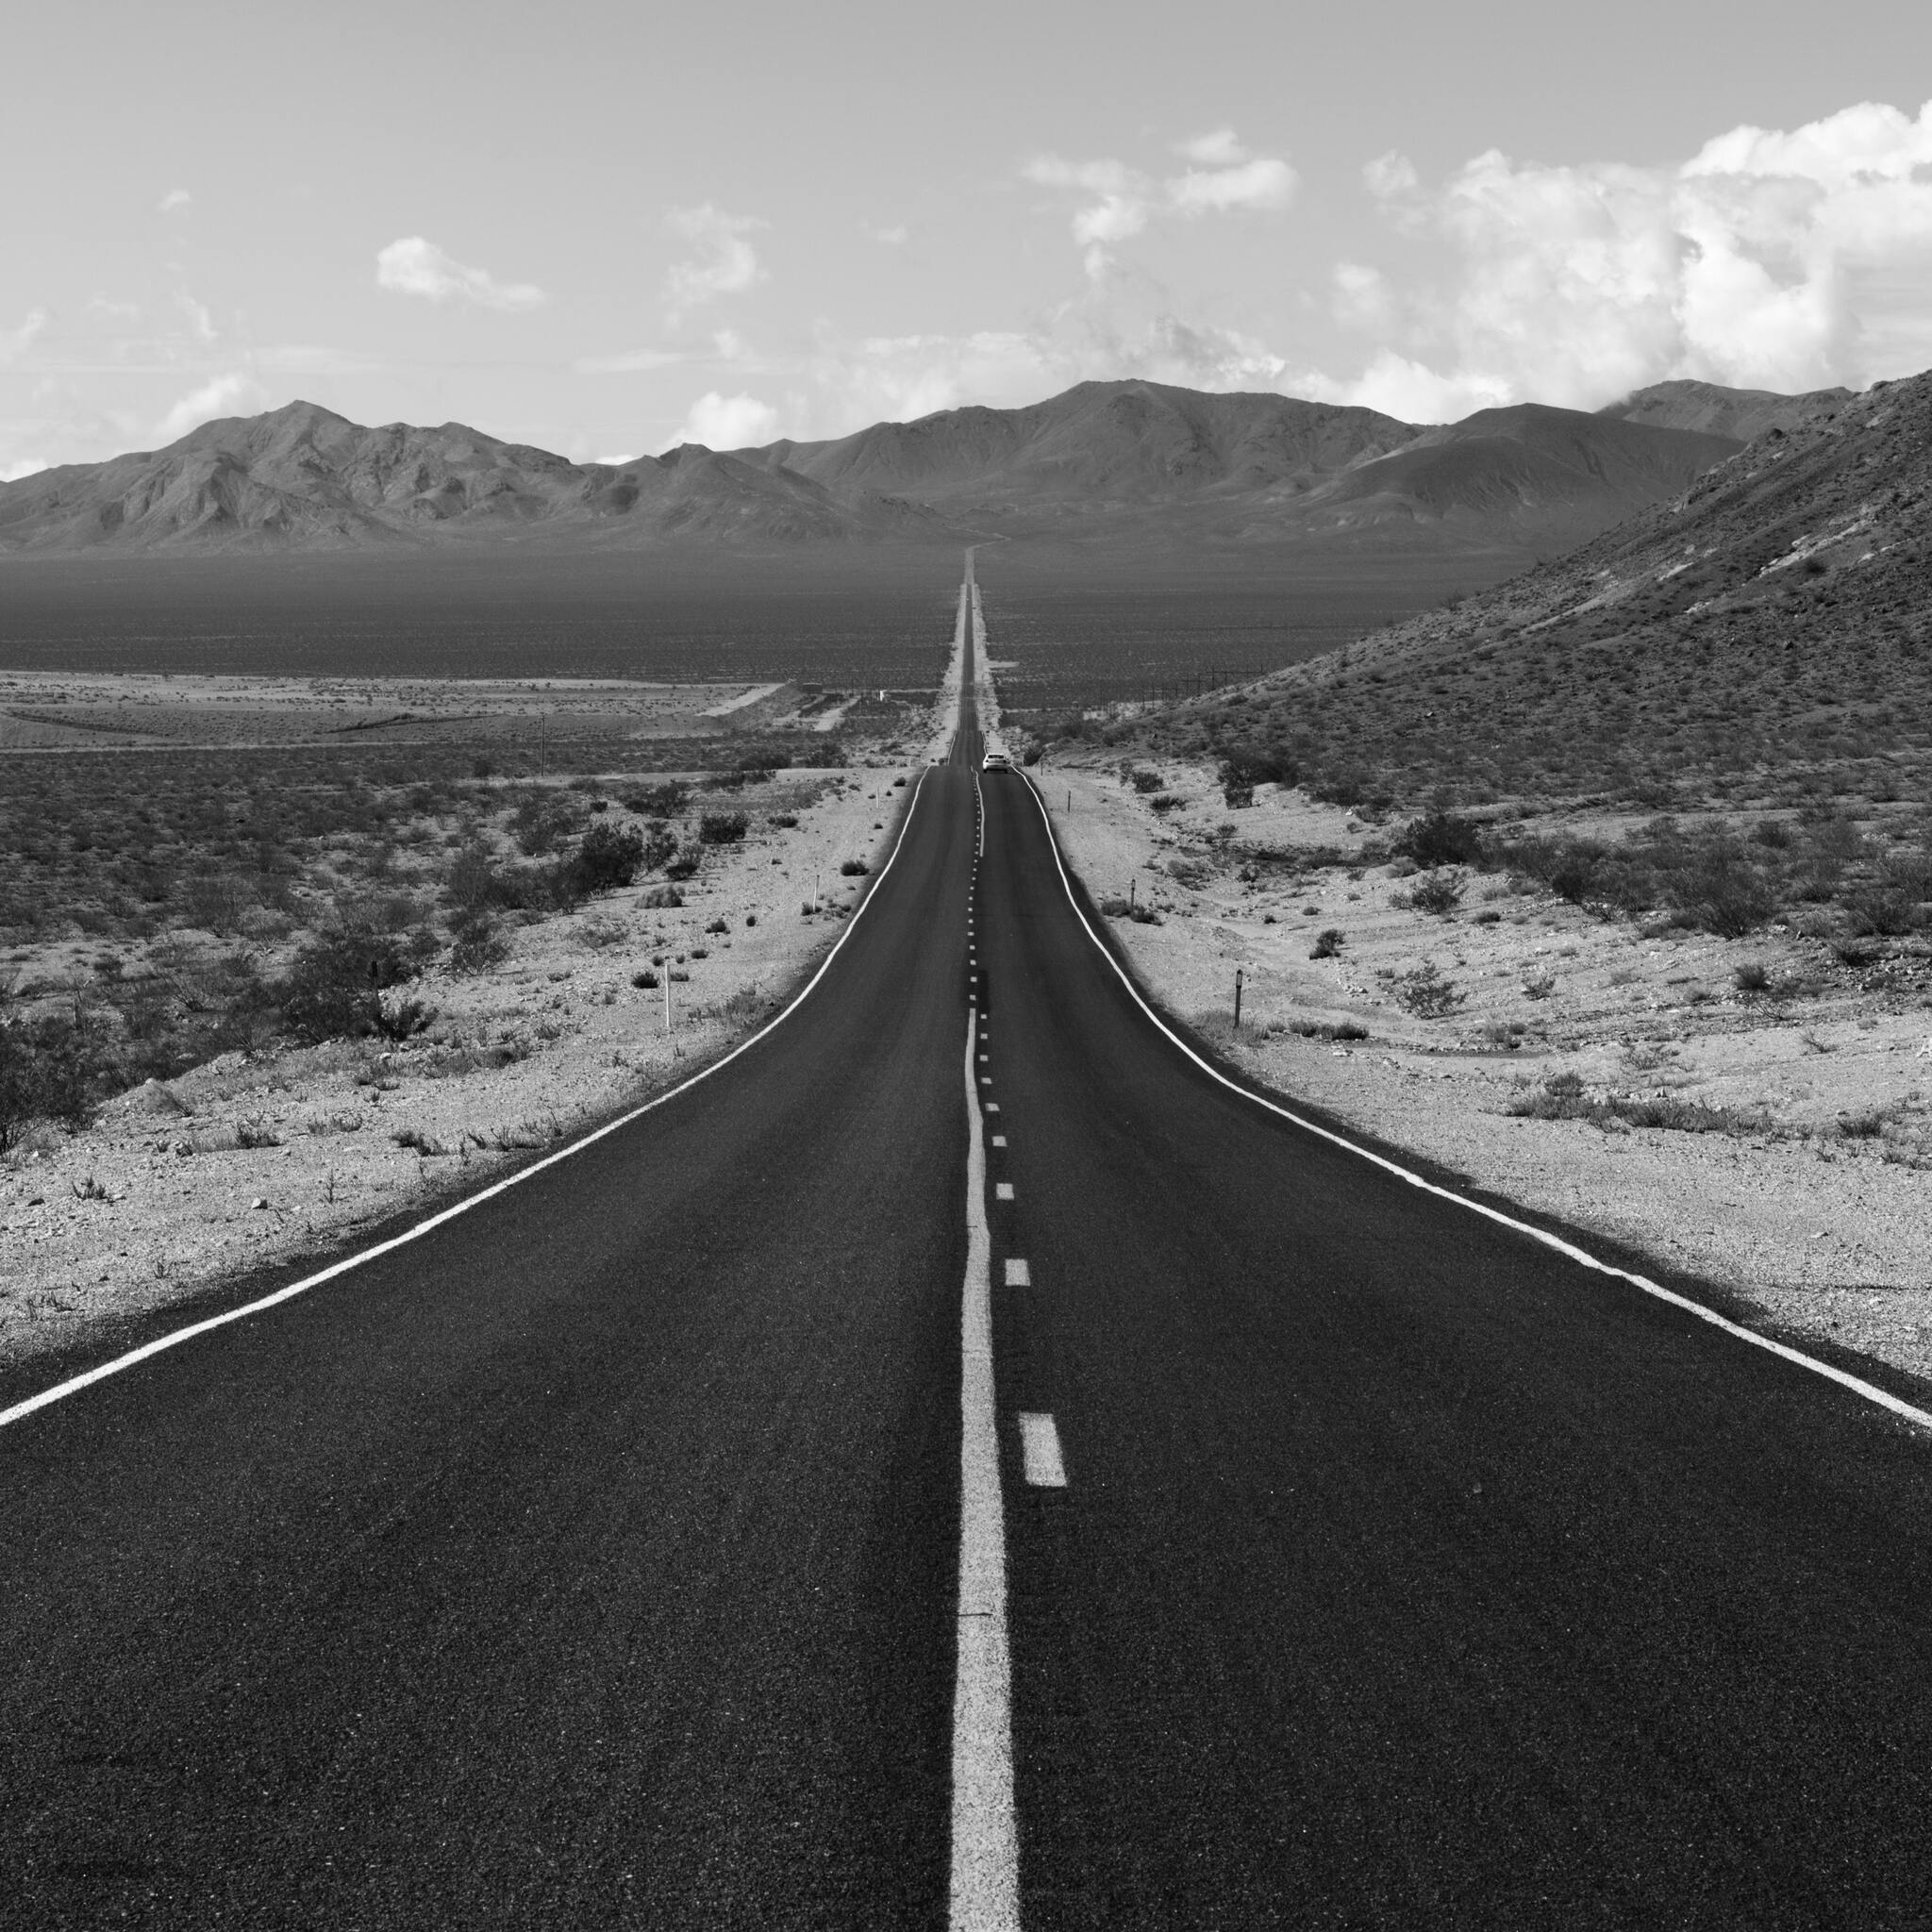
\includegraphics[width=55mm]{image/road_original.jpg}}
    \subfigure[Decompressed image]{\label{fig:road_decompressed}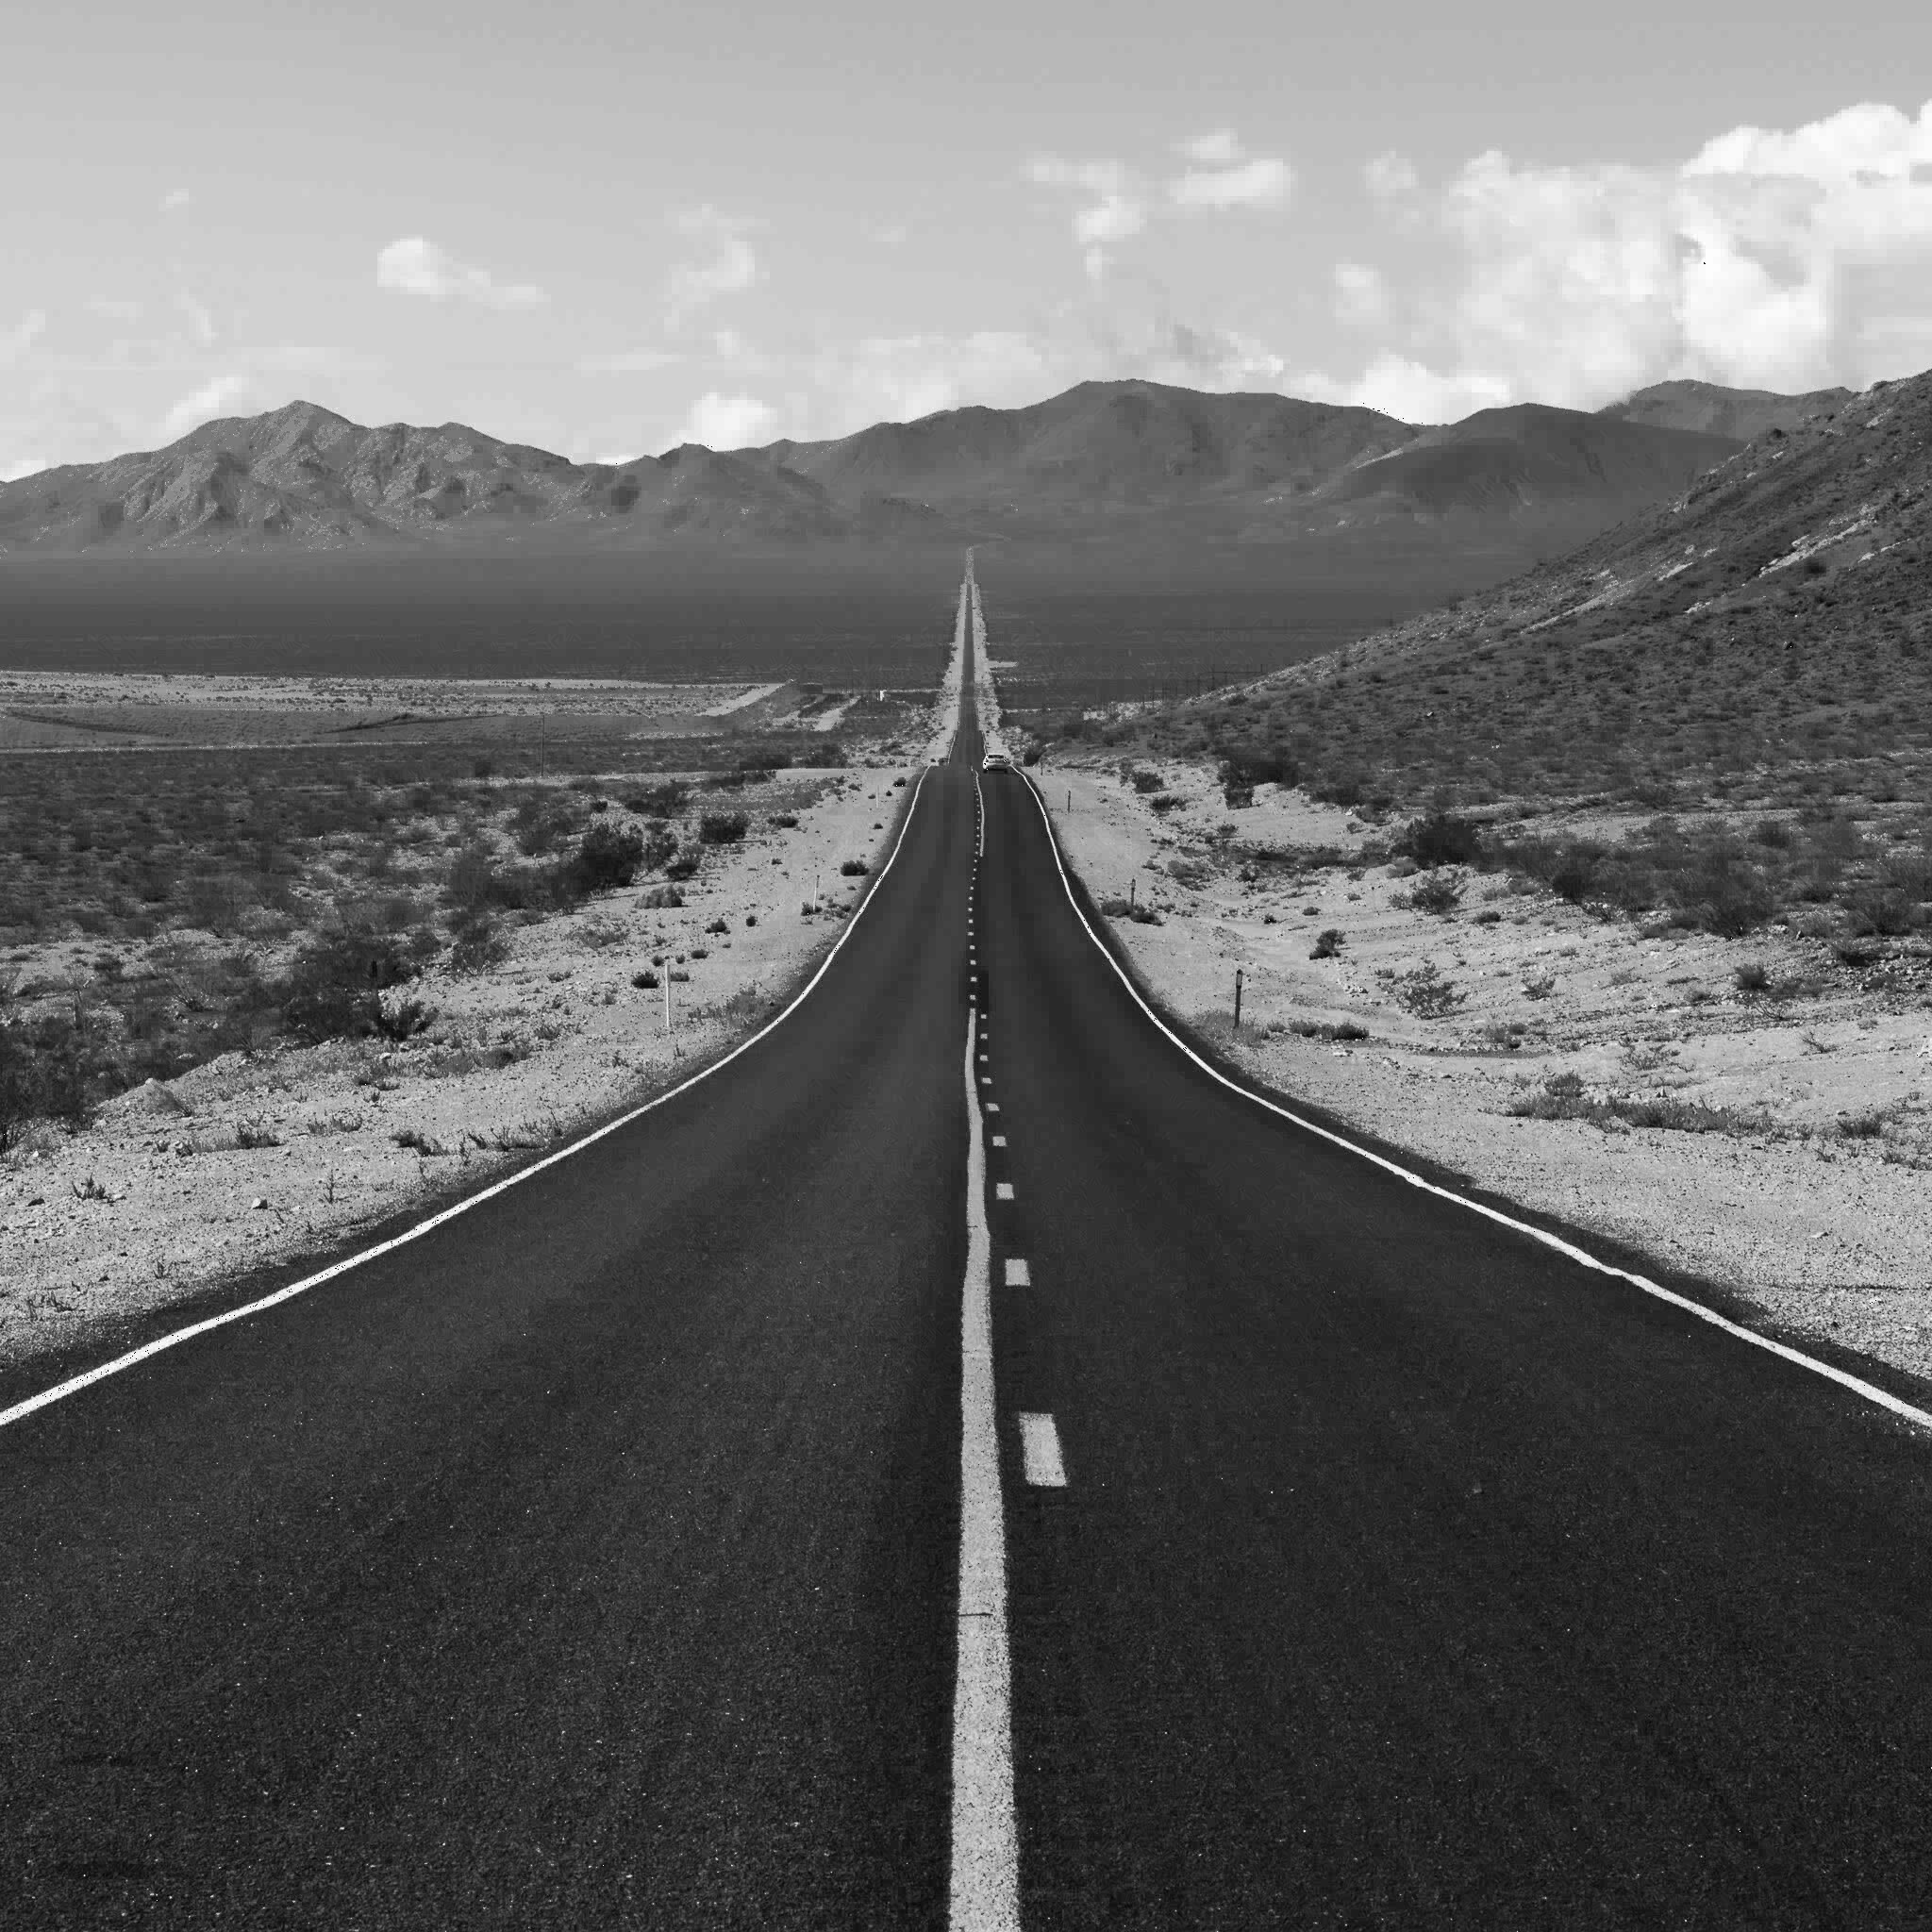
\includegraphics[width=55mm]{image/road_decompressed.jpg}}
    \caption{Our compression algorithm applied to an example image, with a compression rate of 0.82814.}
    \label{fig:compression_road}
\end{figure}

\begin{figure}[ht]
    \centering
    \subfigure[Original image]{\label{fig:cat_original}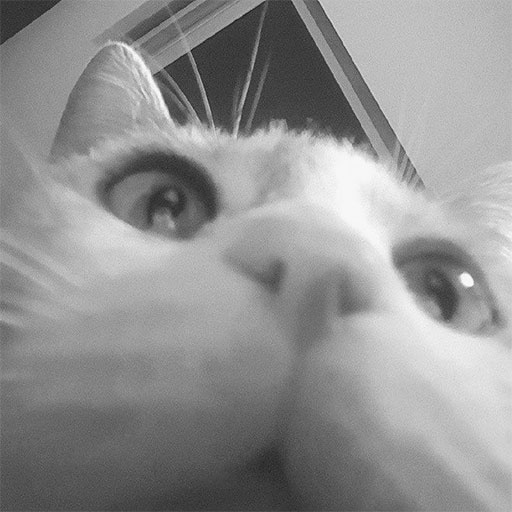
\includegraphics[width=55mm]{image/cat_original.jpg}}
    \subfigure[Decompressed image]{\label{fig:cat_decompressed}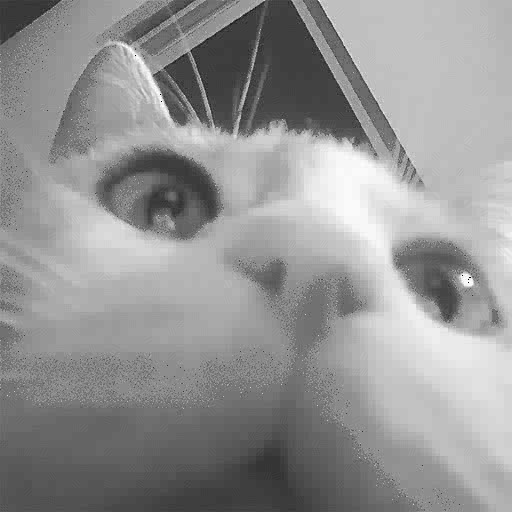
\includegraphics[width=55mm]{image/cat_decompressed.jpg}}
    \caption{Our compression algorithm applied to an example image, with a compression rate of 0.845459.}
    \label{fig:compression_cat}
\end{figure}

The encoded versions of the images have a bitsize of respectively 0.82814 and 0.845459 times that of the original image, achieving a modest decrease in image size. The fact that both the real and the immaginary coefficients have to be stored is a major downside of the DFT over the DCT, as it results in double the bitsize for the same pattern of nonzero values. The compression rate ranges greately in our tests, from 0.09375 for a completely black image (whose reconstructed version is of course the same as the original) to 1.63596 for our worst result.